\subsection{Multiplexación y metodos de acceso}
\begin{figure}[H]
\centering
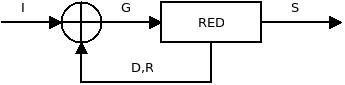
\includegraphics[width=0.5\textwidth]{Imagen/diametodosacceso.jpg}
\caption{Diagrama de Métodos de Acceso}
\end{figure}
\begin{itemize}
\item I: Tráfico. siempre ha de ser menor que 1.
\item G: Tráfico ofrecido a la red.
\item S: Eficiencia de la red.
\item R: Retransmisiones.
\item D: Retardo en la transmisión.
\end{itemize}
I, G, S, R han de estar normalizados a la capacidad de la red. D en cambio ha de estar normalizado a la velocidad de la red. En caso de que no haya congestión S será igual a I. $\sfrac{S}{G}$ expresa la probabilidad media de transmitir paquetes con éxito. $\sfrac{G}{S}$ en cambio el número de retransmisiones medias necesarias para transmitir un paquete con éxito.
\subsubsection{Aloha puro}
\begin{enumerate}
\item Si un terminal quiere transmitir, transmite y espera un ACK del destino.
\item Si no recibe el ACK de confirmación espera un tiempo aleatorio entre uno y k para retransmitir.
\end{enumerate}
\begin{align}
G&=S+R\\
\frac{S}{G}&=e^{-2g}\\
D=(\frac{G}{S}-1)(\frac{k+1}{2}+1+2a+w)+a+1 &
\begin{cases}
a\text{ tiempo de propagación del paquete}\\
w\text{ tiempo de generación del ACK}\\
k\text{ limite máximo de la espera}
\end{cases}
\end{align}
La eficiencia máxima que se puede obtener con ALOHA puro es $S_{max}=0.18$ este valor se produce para G=0.5.\\
\begin{example}[ALOHA puro]
Tenemos un canal de comunicaciones de capacidad 9600bps, y enviamos paquetes de 100 bits. Se sabe que se generan 10.67$\sfrac{paquetes}{segundo}$ y que el tráfico total son 14.4$\sfrac{paquetes}{segundo}$.
\begin{gather*}
C=\frac{9600}{100}\\
D=(\frac{G}{S}-1)(\frac{k+1}{2}+1+2a+w)+a+1\\
I=S=\frac{10.67\sfrac{paq}{s}}{96\sfrac{paq}{s}}=0.11\\
G=\frac{14.4\sfrac{paq}{s}}{96\sfrac{paq}{s}}=0.15\\
\frac{G}{S}=\frac{0.15}{0.11}=1.35\text{ transmisiones por paquete}\\
R=\frac{G}{S}-1=0.35\text{ retransmisiones por paquete}\\
\frac{S}{G}=\frac{0.11}{0.15}=0.74=74\%
\end{gather*}
\end{example}
\subsubsection{Aloha distribuido}
\begin{align}
S=Ge^{-2G(1+a)}\\
D=(e^{-2G(1+a)}-1)(\frac{k+1}{2}+1+2a+w)+a+1
\end{align}
\subsubsection{Aloha ranurado}
El tiempo se divide en ranuras y solo se transmite al comienzo de las ranuras reduciendo el tiempo de colisión.
\begin{align}
S=Ge^{-G}\\
D=(e^{-G}-1)(\frac{k+1}{2}+1.5+2a+w)+a+1.5
\end{align}
La eficiencia máxima que se puede obtener con ALOHA puro es $S_{max}=0.36$ este valor se produce para G=1.\\
\subsubsection{CSMA}
\begin{itemize}
\item Antes de transmitir se escucha el canal.
\item Si no hay nadie transmitiendo se transmite.
\item Si el canal está ocupado:
\subitem No persistente: Se espera un tiempo aleatorio y se escucha el canal. $S=\frac{G}{G+1}$
\subitem 1-persistente: Se escucha hasta que el canal esté libre. $S=\frac{G(1+G)e^{-G}}{G+e^{-G}}$ este tiene una eficiencia máxima del 55\%.
\subitem p-persistente: Se espera con una probabilidad 1-py se transmite con probabilidad p.
\end{itemize}